\documentclass[a4paper,10pt]{article}

\usepackage[utf8]{inputenc}
\usepackage[T1]{fontenc}
\usepackage[french]{babel}
\usepackage{float}
\usepackage{afterpage}
\usepackage[backend=bibtex]{biblatex}
\usepackage{graphicx}
\bibliography{definition}

\usepackage{hyperref}

\title{Régulation d'un système dynamique : application à une serre}
\author{A. Caccia, A. Madeira Cortes, N. Marchant, R. Fontaine}
\date{ }

\begin{document}

\maketitle

\vspace{1cm}

\section{Sujet}

Le but du projet est de modéliser et gérer de façon dynamique l'environnement d'une serre. Plusieurs variables seront analysées et contrôlées: humidité du sol et de l'air, luminosité et température. Ces variables seront récupérées via des capteurs installés dans la serre. \\

Lorsque ces variables dépassent des bornes supérieure ou inférieure données, le logiciel construit activera des dispositifs pour les rétablir entre ces bornes. C'est à dire: \\

\begin{enumerate}
	\item Si la température tombe en dessous de la borne donnée, une résistance chauffante est activée.
	\item Si la température dépasse la borne supérieure donnée, une ventilation est activé.
	\item Si l'humidité de l'air est trop basse, un humidificateur est lancé.
	\item Si l'humidité de du sol est trop basse, un système d'irrigation est enclenché.
	\item La luminosité est régulée par une lampe et un système de volets.\\
\end{enumerate}

\section{Implémentation}

MIMO Multiple Input Multiple Output \\

Algorithme PID, variantes, et autres algorithmes.\\

L'affichage des données sera pris en charge par un visualiseur dédié à l'affichage de données sous forme de graphes: Grafana. Il est possible d'afficher un historique avec des bornes délimitées (en bleu et rouge sur la figure suivante). \\

\newpage

\vspace{-2cm}

\afterpage{%
\thispagestyle{empty}
\begin{figure}[H]
\centering
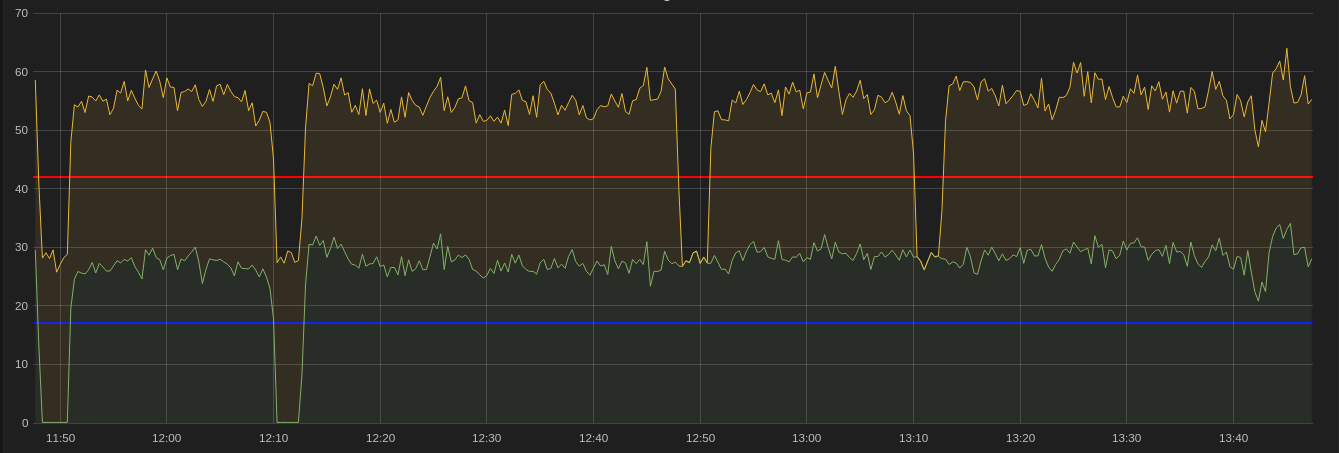
\includegraphics[scale=0.5,angle=90]{figures/Grafana2.png}
\caption{Grafana affichant des données}
\label{grafana}
\end{figure}
}

\newpage

\section{Dispositif de présentation au Printemps des Sciences}

Lors du Printemps des Sciences, nous envisageons de présenter notre projet en exposant une serre où sont cultivées des fraises. \\

L'état des variables contrôlées dans la serre seraient affichées sur un écran, avec un historique visible et les bornes délimitées (comme détaillé dans la partie "Implémentation"). \\

Pour rendre la présentation dynamique et interactive, nous pourrions volontairement perturber le système et celui-ci se stabiliserait tout seul. Nous pourrions par exemple :
\begin{enumerate}
	\item Allumer une lampe et qu'en réaction le système ferme les volets.
	\item Chauffer la serre avec un dispositif externe (par exemple, un sèche-cheveux) pour que la ventilation s'enclenche.
	\item Autres... \\
\end{enumerate}

\section{Bibliographie}

L'article principal auquel nous ferrons référence est \citetitle{Zheying2014}\cite{Zheying2014}. Il présente un cas d'étude très proche du notre en utilisant une version "fuzzy" de l'algorithme PID.\\

\newpage

\printbibliography

\end{document}
